\section{Evaluation}
\label{sec:evaluation}

This section discusses the behaviour of our algorithm in the real
world.

Both for testing and for performance evaluation, we require a test
suite. We started with a carefully crafted, manually produced, suite
of valid and invalid tests. This test suite was constructed by
gathering pairs of types that emerged from examples we have studied
and from programs we have written in FreeST, the programming language
for context-free session
types~\cite{almeida.etal_freest-functional-language}.
% This suite comprised of a total os 169 valid and invalid tests.  The
% primary purpose of this preliminary evaluation step was to confirm
% the algorithm would be able to handle manual examples that we knew
% would emerge from real programs and examples. The algorithm
% succeeded in evaluating all the tests in due time.
The tests produced by this method are, on the one hand, small, and, on
the other hand, lacking diversity.
%
We then turned our attention to the automatic generation of test
cases. Generating pairs of arbitrary (well-formed) types that share no
variables is simple. 
%The difficulty lies in deciding whether two such
%types, independently generated, are bisimilar. Even if an oracle could
%be identified, 
However,
the probability that a randomly generated pair of types
turns out to be equivalent is extremely low. For this reason, we
generate arbitrary pairs of types that are bisimilar by
construction. Theorem~\ref{thm:axioms} naturally induces an algorithm:
given a natural number $n$ (the size of the pair), arbitrarily select
for the base case ($n=0$) one of the pairs in item 1 of the theorem
and for the recursive case ($n\ge1$) one of the pairs in 2--12 items.

\begin{theorem}[Properties of type equivalence]
\label{thm:axioms}
  \begin{enumerate}
    % Congruence
  \item $\skipk \TypeEquiv \skipk$ and $\sharp B \TypeEquiv \sharp B$;
  \item $S;T \TypeEquiv U;V$ if $S \TypeEquiv U$ and $T \TypeEquiv V$;
  \item $\mu X.S \TypeEquiv \mu X.T$ if $S \TypeEquiv T$;
  \item $\star\{\ell_i\colon S_i\}_{i\in I}\TypeEquiv
    \star\{\ell_i\colon T_i\}_{i\in I}$ if $(S_i \TypeEquiv T_i)_{i\in
      I}$;
    % Laws for sequential composition
  \item $S\TypeEquiv T;\skipk$ and $S\TypeEquiv \skipk;T$ if $S \TypeEquiv T$;
  \item $\star\{\ell_i\colon S_i\}_{i\in I};U\TypeEquiv
    \star\{\ell_i\colon T_i;V\}_{i\in I}$ if $(S_i \TypeEquiv T_i)_{i\in
      I}$ and $U \TypeEquiv V$;
  \item $T \TypeEquiv S$ if $S \TypeEquiv T$;
  \item $R;(S;T) \TypeEquiv (U;V);W$ if $R \TypeEquiv U$, $S \TypeEquiv V$, and $T\TypeEquiv W$;
    % Laws for mu-types
  \item
    $\mu X.\mu Y.S \TypeEquiv \mu X.\subs XYT \TypeEquiv \mu Y.\subs
    YXT$ if $S \TypeEquiv T$;
  \item $\mu X.S \TypeEquiv T$ if $S \TypeEquiv T$ and $X\notin\free(S)$;
  \item $\subs UXS\TypeEquiv \subs VXT$  if $S \TypeEquiv T$ and $U \TypeEquiv V$;
  \item $\mu X.S \TypeEquiv \subs{\mu X.T}{X}T$ if $S \TypeEquiv T$.
  \end{enumerate}
\end{theorem}
%
\begin{proof}
  1--3: Bisimulation is a congruence. 4--12: Thiemann and
  Vasconcelos~\cite{thiemann2016context} exhibit the appropriate
  bisimulations. \qed
\end{proof}

For evaluating the algorithm on non-bisimilar pairs we add the 
following five anti-axioms to the list in 
Theorem~\ref{thm:axioms}:
(1) $\skipk \not\sim_\types \sharp B$; \enspace
(2) $\skipk \not\sim_\types X$; \enspace
(3) $\sharp B \not\sim_\types X$; \enspace
(4) $\oplus\{\ell_i\colon S_i\}_{i\in I} \not\sim_\types \&\{\ell_i\colon S_i\}_{i\in I}$; \enspace
(5) $\star\{\ell_i\colon S_i\}_{i\in I} \not\sim_\types \star\{\ell_i\colon S_i\}_{i\in I\cup\{j\}}$,
	where $\ell_j \neq \ell_i$ for all $i$.
%
We generate two types using the same methodology as for the positive case and, 
then, discard the
data collected when the pair turns out to be
bisimilar.
The rationale for this generation of non-bisimilar pairs, rather than
an arbitrary and independent generation of types, relies on the reality that 
the compiler faces most often.
For testing, however, we rely on manually crafted tests, given that a
solution based on anti-axioms does not always work: note that
bisimulation for
context-free session types is such that there are types
$S \not\bisim T$ such that $\mu X.S \bisim \mu X.T$ (just think of
$!\intk;X;X$ and $!\intk;X$).


We used QuickCheck~\cite{DBLP:conf/icfp/ClaessenH00} to generate two test
suites. That for bisimilar pairs is constructed based on
Theorem~\ref{thm:axioms}, whereas the construction of non-bisimilar tests
rely on Theorem~\ref{thm:axioms} plus the anti-axioms above. Both test suites
comprise 2000 entries, featuring types with
a number of nodes (in the syntax tree) ranging from 1 to 200.
We consider the size of a pair of types as the maximum number of nodes in the 
syntax tree,
chosen among the two types. 
%The test suites have diversity: 100 pairs whose
%size is between 1 and 10 nodes, 100 pairs with 11 to 20 nodes, and so on.

The base algorithm described in the previous section turns out to
behave quite poorly (see Figure~\ref{fig:distribution}). We then implemented the
following variants:
%
\begin{enumerate}
\item \emph{Eliminating redundant productions in the grammar.}
  Since the size of the expansion tree depends, among other
  things, on the number of productions in the grammar, generating smaller 
  grammars seems a promising optimisation. Rather than blindly adding a
  new production $Y \rightarrow \vec Z$, we look, in the set of
  productions, for a production $W \rightarrow \vec X$ 
  syntactically equal to the former, up to renaming of non-terminal
  symbols.
  In this case, we add no new production and return
  non-terminal~$W$ instead. To find~$W$, we look for the least
  fixed-point of the transitions in the languages generated by
  $\vec Z$ and $\vec X$ and compare them.
  This optimisation does not compromise the results 
  of soundness, completeness, nor termination.
  \item
  \emph{Using a filter rule that removes nodes with hopeless pairs.} A
  filter rule ensures that nodes composed by pairs of types with
  different norms (if normed) are removed from the expansion tree,
  since these types are not equivalent.  
  The filter rule
  preserves the results of soundness, completeness, and termination.
  \item
  \emph{Using a double-ended queue to prepend promising children.} A
  double-ended queue allows prioritizing nodes with potential to reach
  an empty node faster.  The algorithm prepends (rather than appends)
  empty nodes or nodes whose pairs $(\vec X, \vec Y)$ are such that
  $|\vec X|\leq 1$ and $|\vec Y| \leq 1$.
  This procedure does not compromise soundness, completeness, nor
  termination because the number of terminal symbols is finite and the 
  algorithm takes advantage of the reflexive and congruence 
  rules to remove previously visited nodes from the queue.
  \item
  \emph{Iterating the simplification stage until a fixed point is
    reached.} Iterating the simplification procedure on a given node
  $N$, the algorithm computes the simplest possible children nodes
  derived from $N$. We showed that the simplification function that
  results from applying the reflexive, congruence, \BPA, and filter
  rules, has a fixed point in the complete partial ordered set of
  pairs node-ancestors, where the set of ancestors is fixed.
  This optimisation preserves soundness, completeness and termination.
\end{enumerate}

To better understand how the algorithm performs in practice, we teste
all the optimisations and their combinations. We evaluate each variant 
1--4 individually (denoted
by B1--B4) and all their combinations. For instance, we denote by B124
the variant obtained from combining optimisations 1,2, and 4 above.
B stands for the base algorithm, $\BisimT$.
%
  We implemented the base algorithm and its
  variants %described by the function $\BisimT$
  in Haskell, using the Glasgow Haskell Compiler (version 8.6.5). % We also
  % implemented the optimisations 1-4 above.
  The evaluation was conducted on a machine with an Intel Core i7-6700K at
  4.2GHz and 8 GB of RAM running Arch Linux; tests were run under a timeout
  of 2 minutes.

% For B0 we had 5 tests exceeding the timeout, for B1--B4 the number of timeouts
% ranged from 1 to 12, for B12 we had 2 timeouts, whereas for B1234 all tests
% ran in less than 30 minutes. 
%
%\begin{table}
%\centering 
%	\begin{tabular}{ |c|c|c|c| }
%	 \hline
% 		Version ID & Version description & Bisimilar test suite & Not bisimilar 
% 		test suite \\ 
% 		 \hline
%	 	B0 & \text { base case}& 5 & 0 \\  
%	 	B1 & \text { reuse productions}& 2 & 1 \\ 
%	 	B2 & \text { use double-ended queue}& 6 & 0 \\ 
%	 	B3 & \text { use filtering}& 12 & 0 \\
%	 	B4 & \text { iterate simplification}& 4 & 0 \\
%	 	B12 & \text {case B1 + case B2}& 3 & 1 \\   
%	 	B123 & \text {case B12 + case B3}& 7 & 1 \\
%	 	B1234 & \text {case B123 + case B4}& \bf{1} & \bf{1} \\ 
%	 	 \hline  
%	\end{tabular}
%	\caption{Number of timeouts for each optimisation.\label{table:timeouts}}
%\end{table}
%
%
Figure~\ref{fig:distribution} depicts the distribution of the execution
times (in $ms$) for both test suites and all variants. We observe that 
the behavior of negatives tests is roughly the same in all variants. However,
the execution time for the positive tests differ from variant to variant. These
differences mainly depend on the trade-off between the computational
effort underlying each optimisation and the efficiency they bring to
deciding the equivalence of grammars. 
Figure~\ref{fig:timeouts} shows the number of timeouts for each variant.
The base case, B, has 301 positive tests whose execution time
exceeds 2 minutes. Some variants perform better than the base case, 
some others perform worst, again mainly due to the trade-off between the 
effort to compute the optimisations and the benefit they bring.
For the negative tests, we do not have any timeouts.
Variant B14, resulting from combining optimisations 1 and 4, 
performs better than all others, presenting a median of 1.4 milliseconds
for the positive tests and 7 timeouts. 
The distribution of execution time of B14 by the size of the input
types is depicted in Figure~\ref{fig:numberOfNodes}.
As expected, the execution time increases considerably with the number of nodes.
%
Although we have carried out tests with a
fairly large number of nodes in their abstract syntax trees, we remark
that, when used in a compiler, the algorithm will mostly come across
types with a reduced number of nodes.


% \begin{figure}[t]
%     \centering
%     \subfloat[Distribution of the execution time]{\includegraphics[height=.5\textwidth]{img/old_distribution_boxplot}}%
%     \subfloat[Execution time per number of nodes]{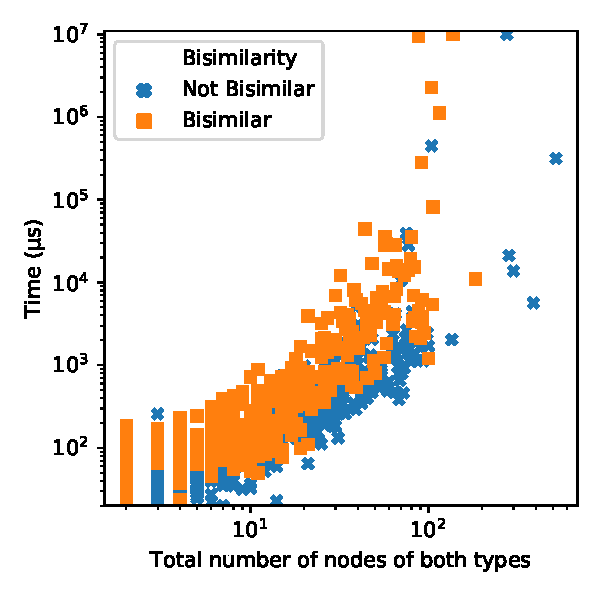
\includegraphics[height=.5\textwidth]{img/nodes_time_B1234}}%
%     \caption{The test suite composed by equivalent pairs of types is represented in orange and the
%     test suite with non-equivalent pairs of types is represented in blue. Time 
%     in microseconds, $\mu s$. Both scales are logarithmic.\\
%     (a) Distribution of execution time of function $\BisimT$ for both test suites.\\
%     (b) Distribution of execution time of function $\BisimT$ per total number of nodes 
%     in the abstract syntax trees of the types.}%
%     \label{fig:results}%
%   \end{figure}

  
\begin{figure}[t]
%\centering
  \subfloat[Distribution of the execution time per variant]{
    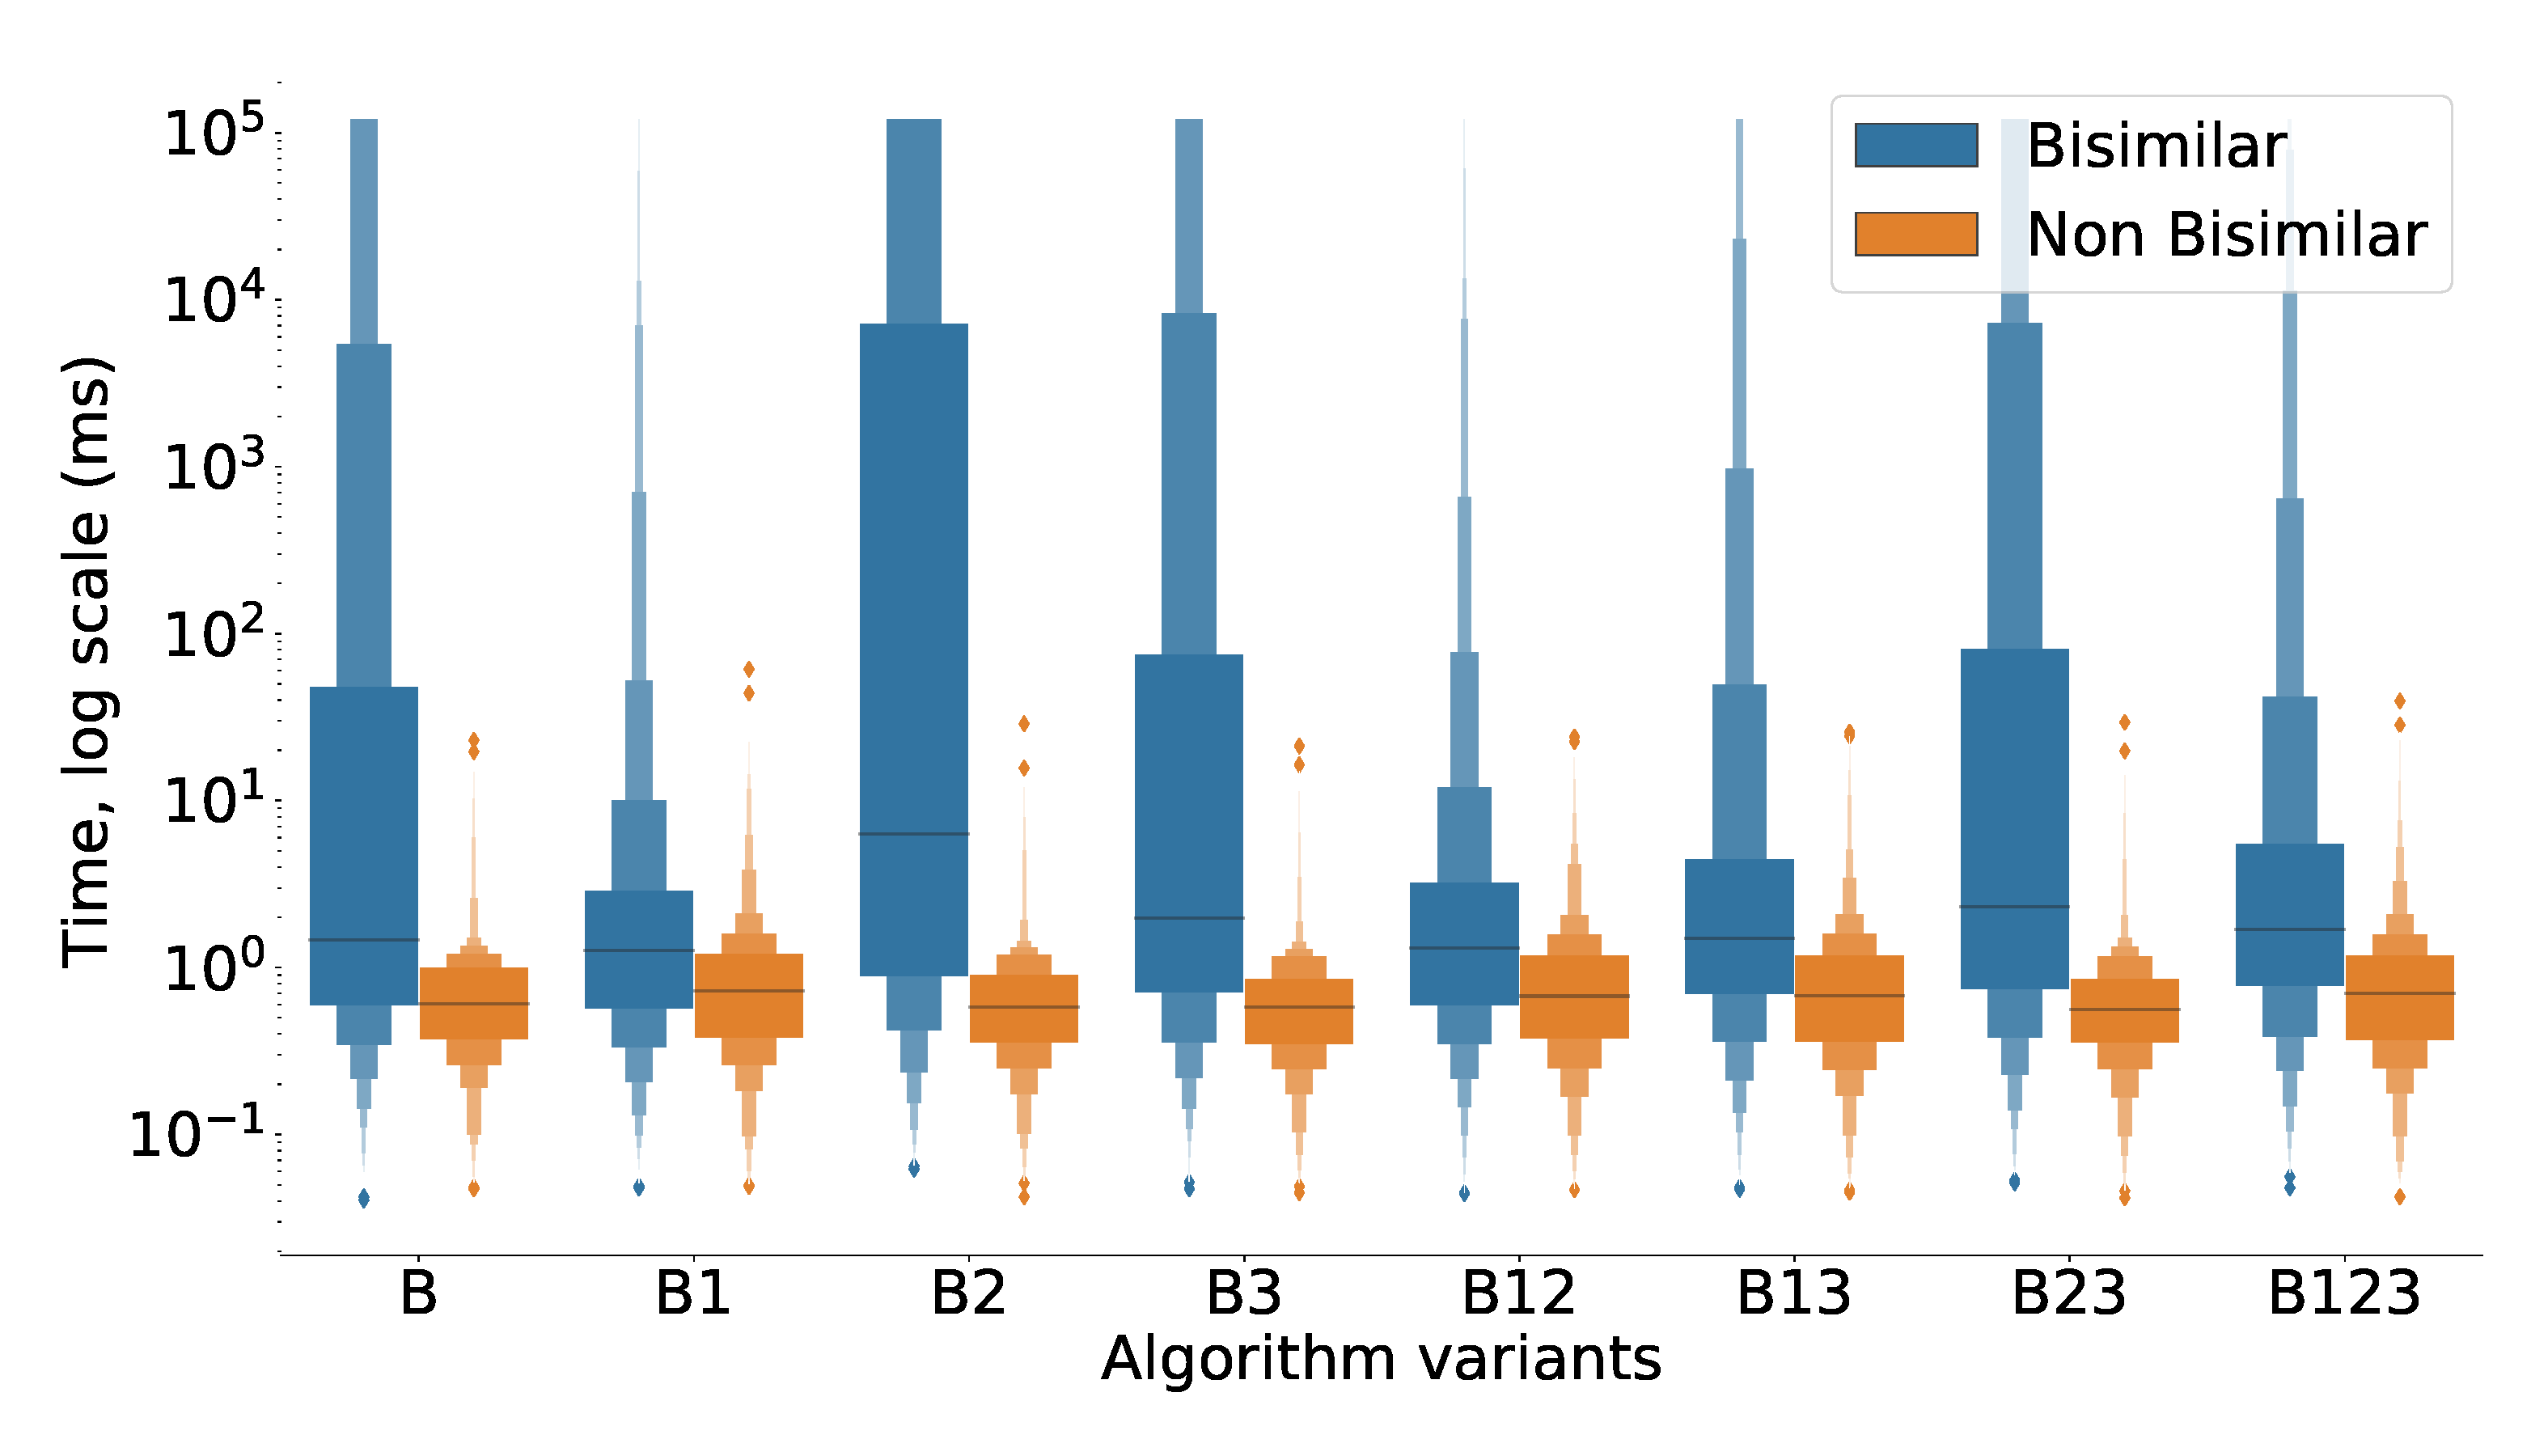
\includegraphics[width=0.9\textwidth]{img/distribution_boxplot}
    \label{fig:distribution}}
  
  \subfloat[Number of timeouts per variant]{ 
    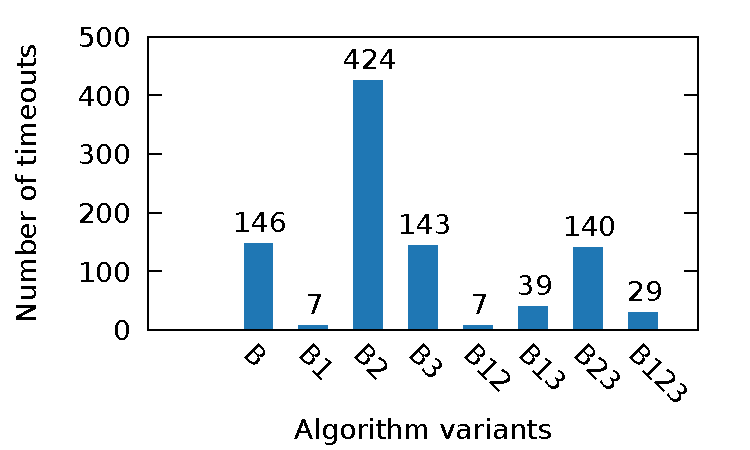
\includegraphics[height=.3\textwidth]{img/timeouts}
    \label{fig:timeouts}}
  %
  \subfloat[Execution time per number of nodes]{
    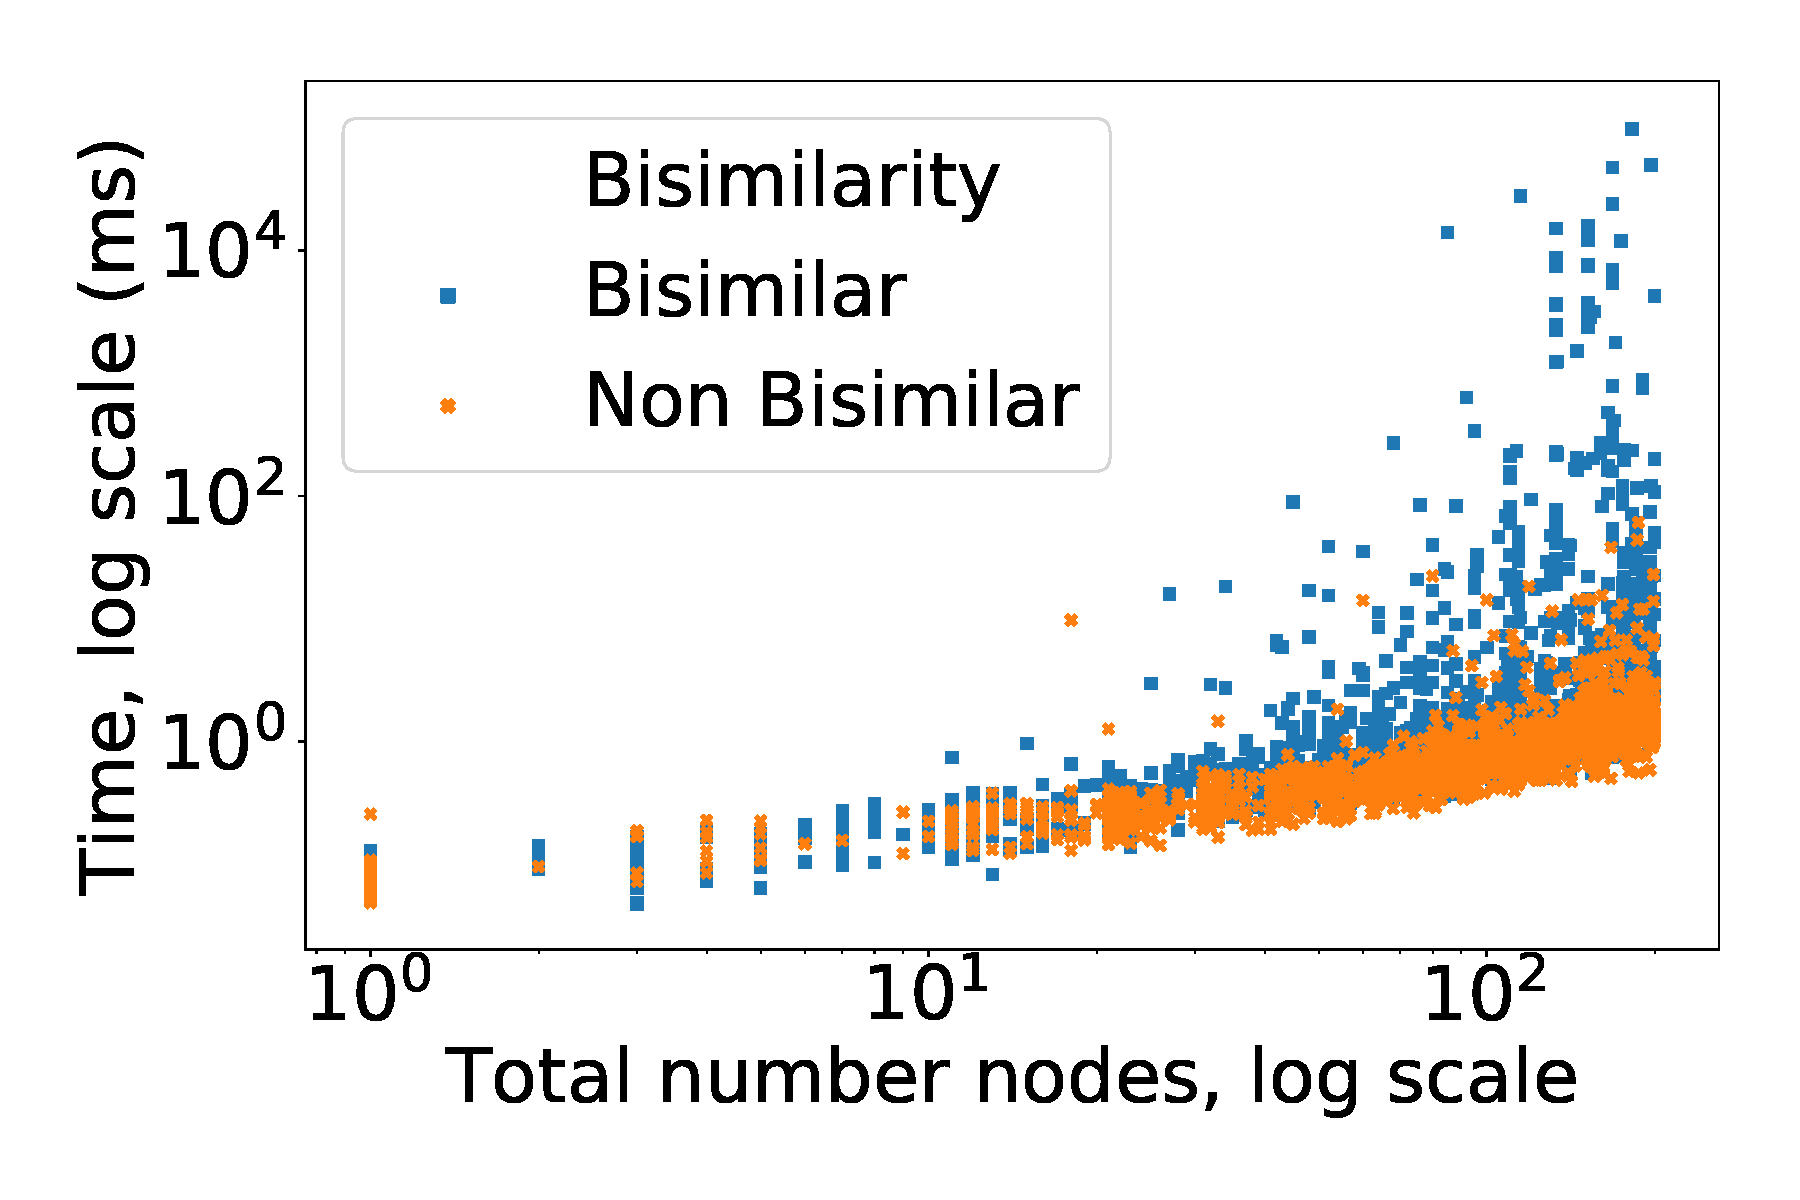
\includegraphics[height=.32\textwidth]{img/nodes_time}
    \label{fig:numberOfNodes}
  } 
\caption{The test suite composed by equivalent pairs of types is represented in blue and the
  test suite with non-equivalent pairs of types is represented in orange. Time is in
  milliseconds. Both scales of \ref{fig:distribution} and \ref{fig:numberOfNodes} are logarithmic and
  the scale of \ref{fig:timeouts} is linear.}
\label{fig:results}
% \caption{The test suite composed by equivalent  pairs o f types is represented in orange and the
%     test suite with non-equivalent pairs of types is represented in blue. Time 
%     in microseconds, $\mu s$. Both scales are logarithmic.\\
%     (a) Distribution of execution time of function $\BisimT$ for both test suites.\\
%     (b) Distribution of execution time of function $\BisimT$ per total number of nodes 
%     in the abstract syntax trees of the types.}
% \label{fig:subfigureExample}
\end{figure}

%\noindent
%\begin{minipage}[b]{0.49\textwidth}
%   {\small 
%  \centering
% 	\begin{tabular}{ |c|c|c| }
%	 \hline
% 		Version &  {\color{orange}Bisimilar} & {\color{MidnightBlue}Not bisimilar}  \\ 
% 		 \hline
%	 	B0 & 5 & 0 \\  
%	 	B1 &  1 & 0 \\ 
%	 	B2 & 6 & 0 \\ 
%	 	B3 &  12 & 0 \\
%	 	B4 &  4 & 0 \\
%	 	B12 &  2 & 0 \\   
%	 	B123 &  6 & 0 \\
%	 	B1234 &  \textbf{0} & \textbf{0} \\ 
%	 	 \hline  
%	\end{tabular}\vspace*{6mm}
%	\captionof{table}{Number of timeouts for each optimisation and for both test 
%	suites.\label{table:timeouts}\vspace*{4mm}}
%	}
%	\end{minipage}
%	\hfill
%\begin{minipage}[b]{0.49\textwidth}
% {\small 
%\centering
%    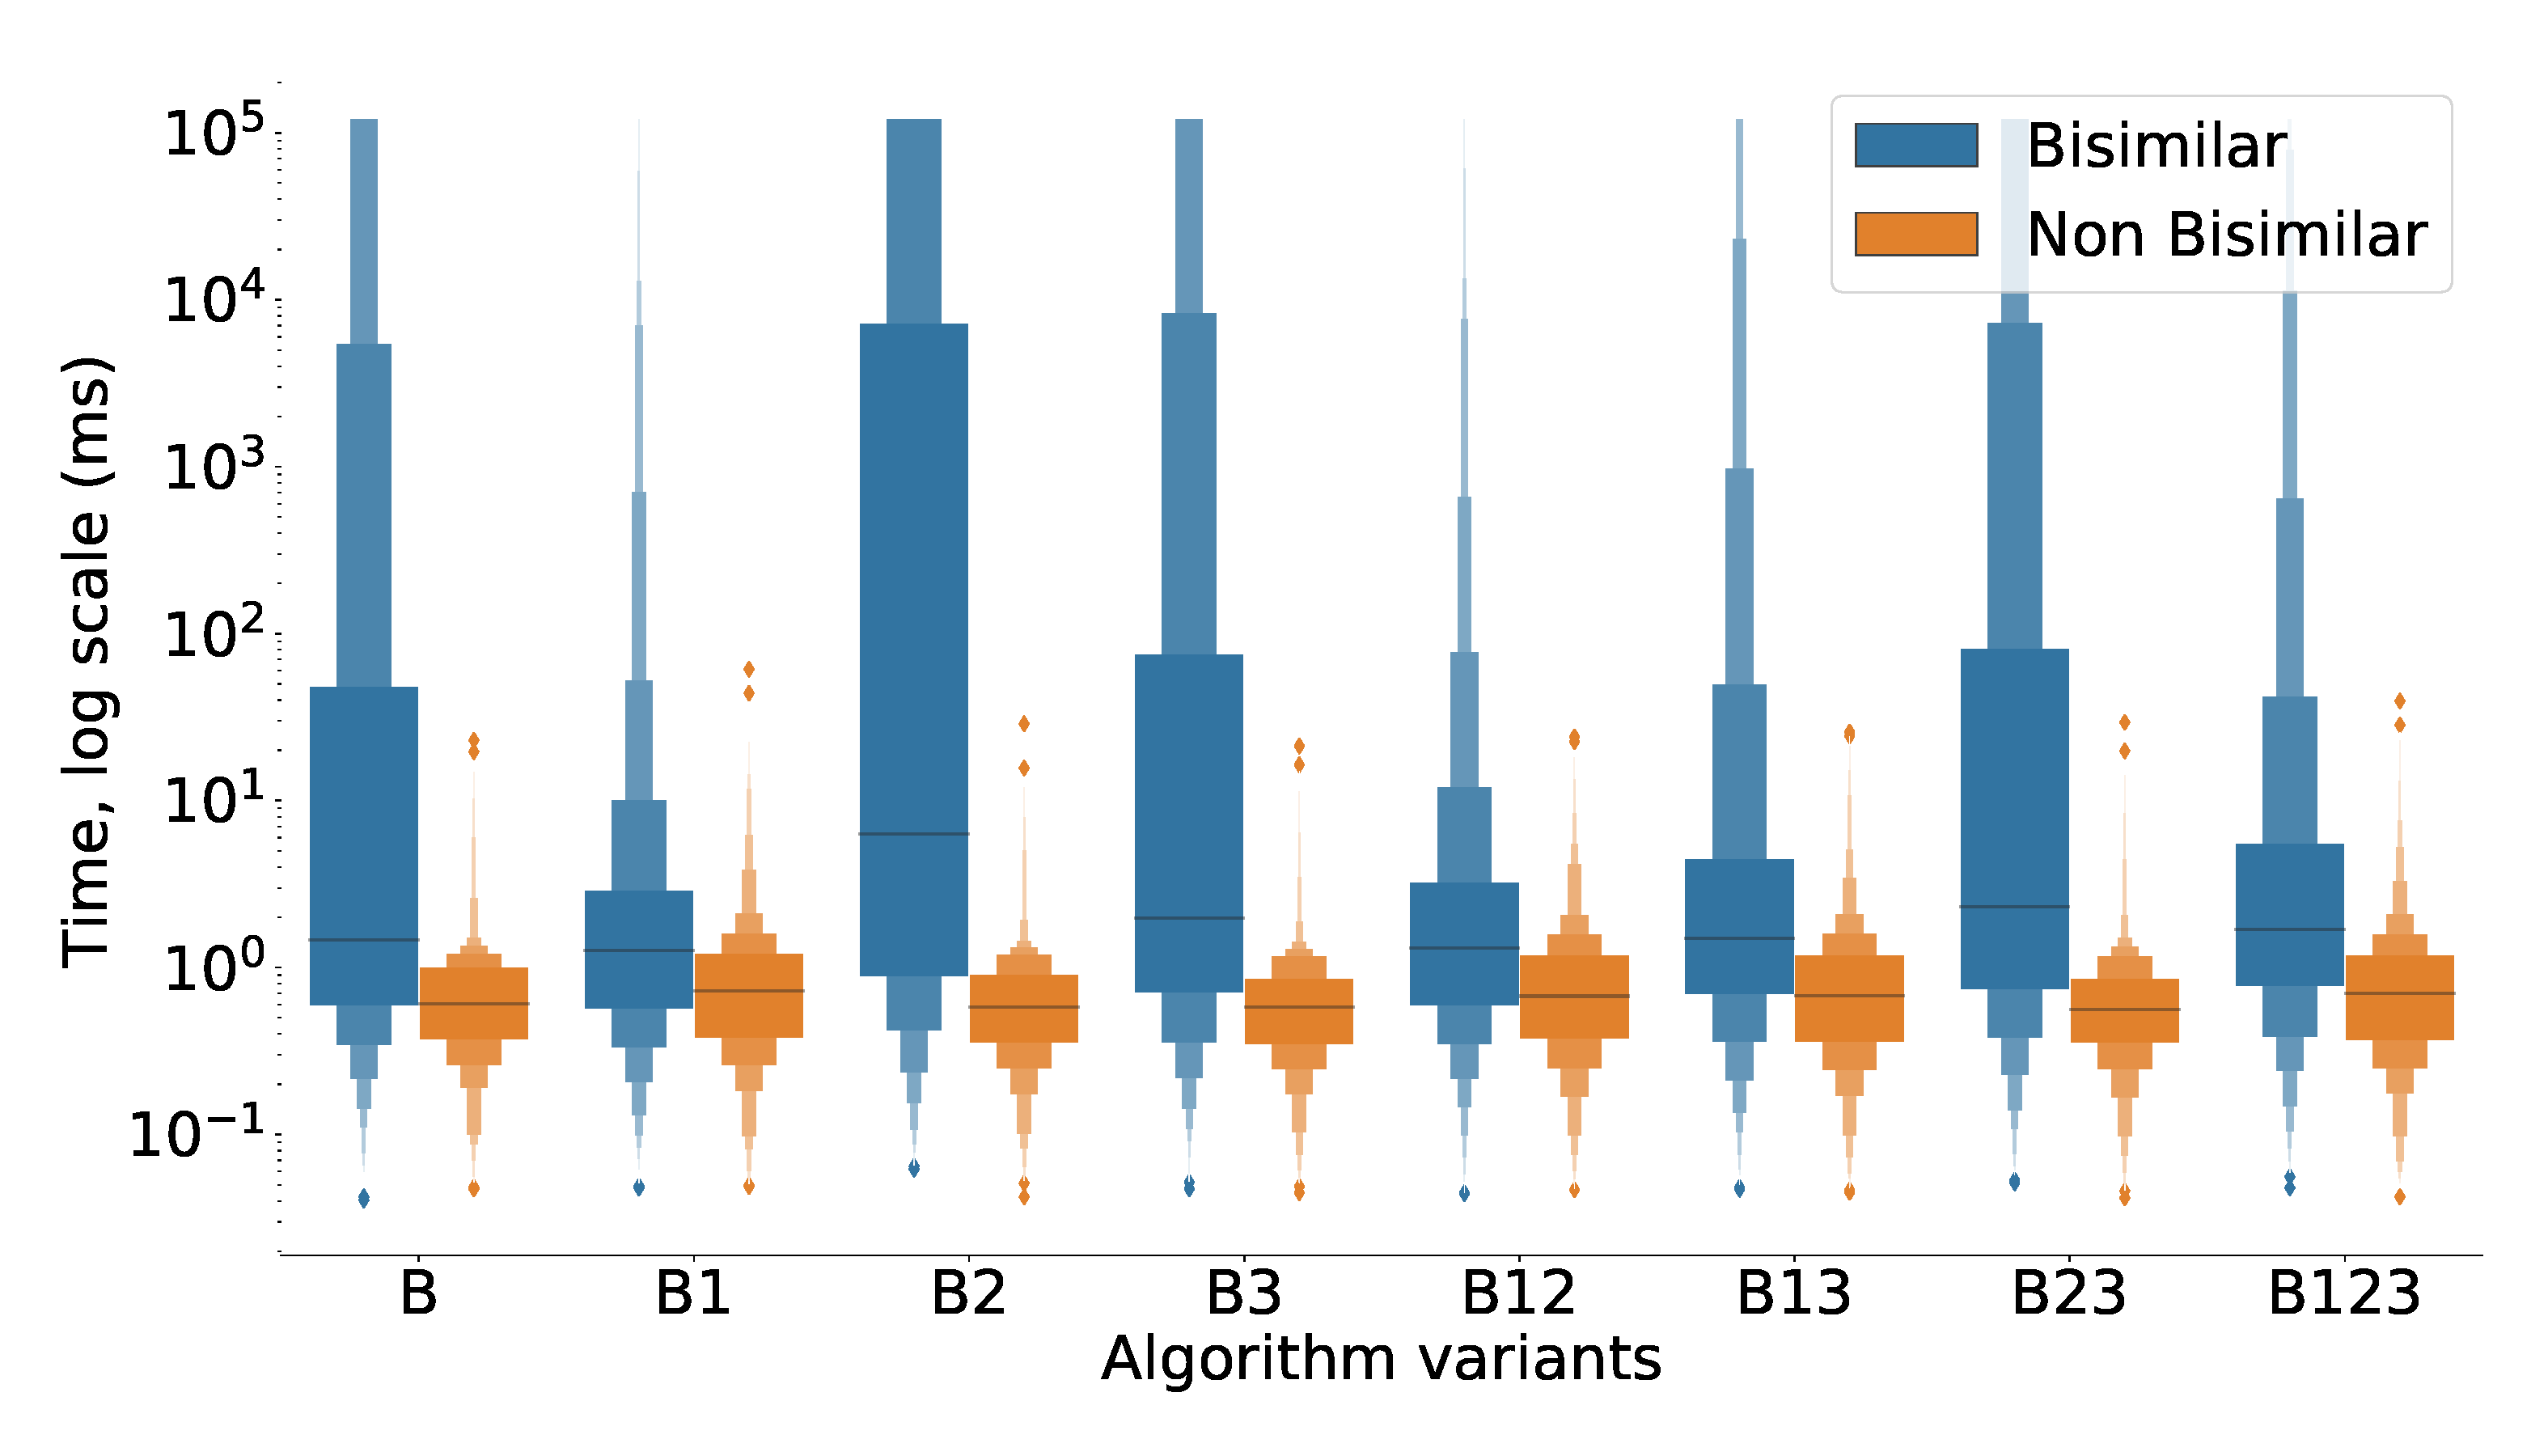
\includegraphics[height=.85\textwidth]{img/distribution_boxplot}%
%    \captionof{figure}{Distribution of execution time of function $\BisimT$ for both test suites. 
%    Both scales are logarithmic.\label{fig:results}}}
%    %\caption{Distribution of the execution time. \label{fig:results}}
%\end{minipage}

%%% Local Variables:
%%% mode: latex
%%% TeX-master: "main"
%%% End:
